\subsection{DOP 26 Постановка задачи дискретной оптимизации. Метод ветвей и границ. Задача целочисленного линейного программирования.}

Постановка задачи дискретной оптимизации: найти $\min_{x \in X} f(x)$, где $X$ - конечно или счетно (мн-во допуст. значений перем. $x$), в постановке м.б. и нахождение и $\max$

\textbf{Метод ветвей и границ}

Две процедуры: ветвление и нахождение оценок (границ), т.е. для того чтобы МВГ работал, нужны: 

1) метод разбиения задачи на подзадачи 

2) функция оценки решения.

Процедура ветвления состоит в разбиении множества допустимых значений переменной $x$ на подобласти (подмножества) меньших размеров. 
Процедуру можно рекурсивно применять к подобластям. 
Полученные подобласти образуют дерево, называемое \textbf{деревом поиска} или деревом ветвей и границ. Узлами этого дерева являются построенные подобласти (подмножества множества значений переменной $x$). 
Процедура нахождения оценок заключается в поиске верхних и нижних границ для решения задачи на подобласти допустимых значений переменной $x$. В основе МВГ лежит следующая идея: если нижняя граница значений функции на подобласти $A$ дерева поиска больше, чем верхняя граница на какой-либо ранее просмотренной подобласти $B$, то $A$ может быть исключена из дальнейшего рассмотрения (правило отсева). 
Обычно минимальную из полученных верхних оценок записывают в глобальную переменную $m$; любой узел дерева поиска, нижняя граница которого больше значения $m$, может быть исключен из дальнейшего рассмотрения (закрыт). 
Если нижняя граница для узла дерева совпадает с верхней границей, то это значение является минимумом функции и достигается на соответствующей подобласти.

\textbf{Основная задача линейного программирования} (озЛП) $(c_1, c_2, \dots , c_n)$, найти 
$$\max_{x \in R,~Ax \leqslant b} \langle c, x \rangle.$$

\textbf{Каноническая задача ЛП}: 
$$\max_{Ax = b,~x \geqslant 0} \langle c, x \rangle.$$

Формально данные задачи не являются дискретными, но они могут быть сведены к перебору конечного числа угловых точек (вершин полиэдра, задающего ограничения) на основании принципа граничных решений:

Если задача имеет решение, то найдется такая подматрица $A_I$ матрицы $A$, что любое решение системы уравнений $A_Ix = b_I$ реализует максимум.

Для задачи целочисленного ЛП на переменные накладывается требование их принадлежности мн-ву целых чисел:

$$\max_{x \in Z,~Ax \leqslant b} \langle c, x \rangle.$$

Пример: Найти $\max Z = 5x_1 + 6x_2$ при ограничениях $x_1+x_2 \leq 50$, $4x_1+7x_2 \leq 280$, $x_1,x_2 \geq 0$ - целые

Общая схема МВГ для примера: строим области ограничения $x_1 \leq -x_2+50$ и $x_1 \leq - \frac{7}{4}x_2+70$,
точка пересечения $x1=\frac{70}{3}=23.333, x2=\frac{80}{3}=26.667, Z=5*\frac{70}{3}+6*\frac{80}{3}=276.667$ -- не явл.целочисл. 
Решение лежит внутри области, заданной ограничениями. 
Мы проверяем другие конечные точки, проводя линию, задающие целочисл ограничения для $x_1, x_2$ по области. 
Выбираем переменную для ветвления (иногда выбор важен, тк в некоторых примерах придется рассмотреть больше/меньше ветвей), 
в данном случае $x_2$ становится параметром для МВГ: берем область $x_2 \leq 26$, находим точку пересеч. 
с границей ${x_1=24, x_2=26, Z=276}$ - получили целочисл. решение. 
Сама точка называется текущим целочисленным рекордом или просто рекордом, а оптимальное значение целочисленной задачи — текущим значением рекорда. 
Это значение является нижней границей оптимального значения исходной задачи и с ним будем сравнивать все след. значения Z, 
переходим к след. ветви $x_2 \geq 27 \Rightarrow \{x_1=22.75, x_2=27, Z=275.75\}$ --- нецелочисл. и $\leq$ рекорда, ветвимся теперь по $x_1$: 
строим $x_1 \leq 23 \Rightarrow \{x_1=23, x_2=26.857, Z=276.142 \}$ > рекорда, теперь внутри этой ветви нужно разветвиться по $x_2 \leq 26$ и $x_2 \geq 27$, 
внутри этих ветвей получим значения целевой функции меньшие или равные рекорду. 
Пробуем ветвь по $x_1:$ $x_1 \geq 24$ и приходим к $Z=276 \leq$ рекорда, в данную ветвь не заходим.


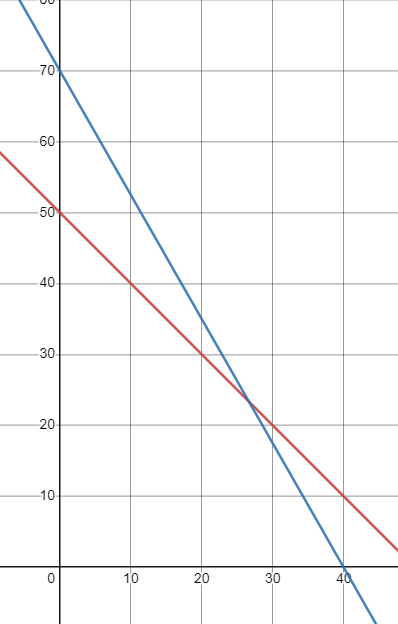
\includegraphics[scale=0.7]{pics/dop27_1.png}

Ограничения, сюда добавляем также ограничение текущей ветки


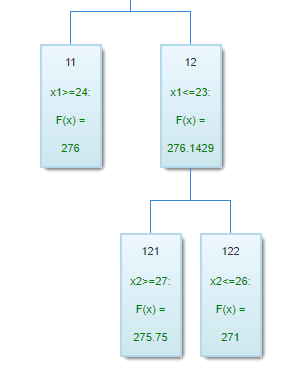
\includegraphics{pics/dop27_2.png}

Ветвление по $x_1$

% -------- source --------
\bigbreak
[\cite[page 69-96]{replace_me}]